% 方法章节
% 说明：
% 1. 本文件设计为被主文档 \input{} 进来使用。
% 2. 内容来源于 04_paper.md 的 Method 部分。
% 3. 这里只做 Markdown 到 LaTeX 的语法迁移与公式环境适配。

% 让系统流程图出现在 Method 标题所在页的页顶。

\begin{figure*}[!t]
    \centering
    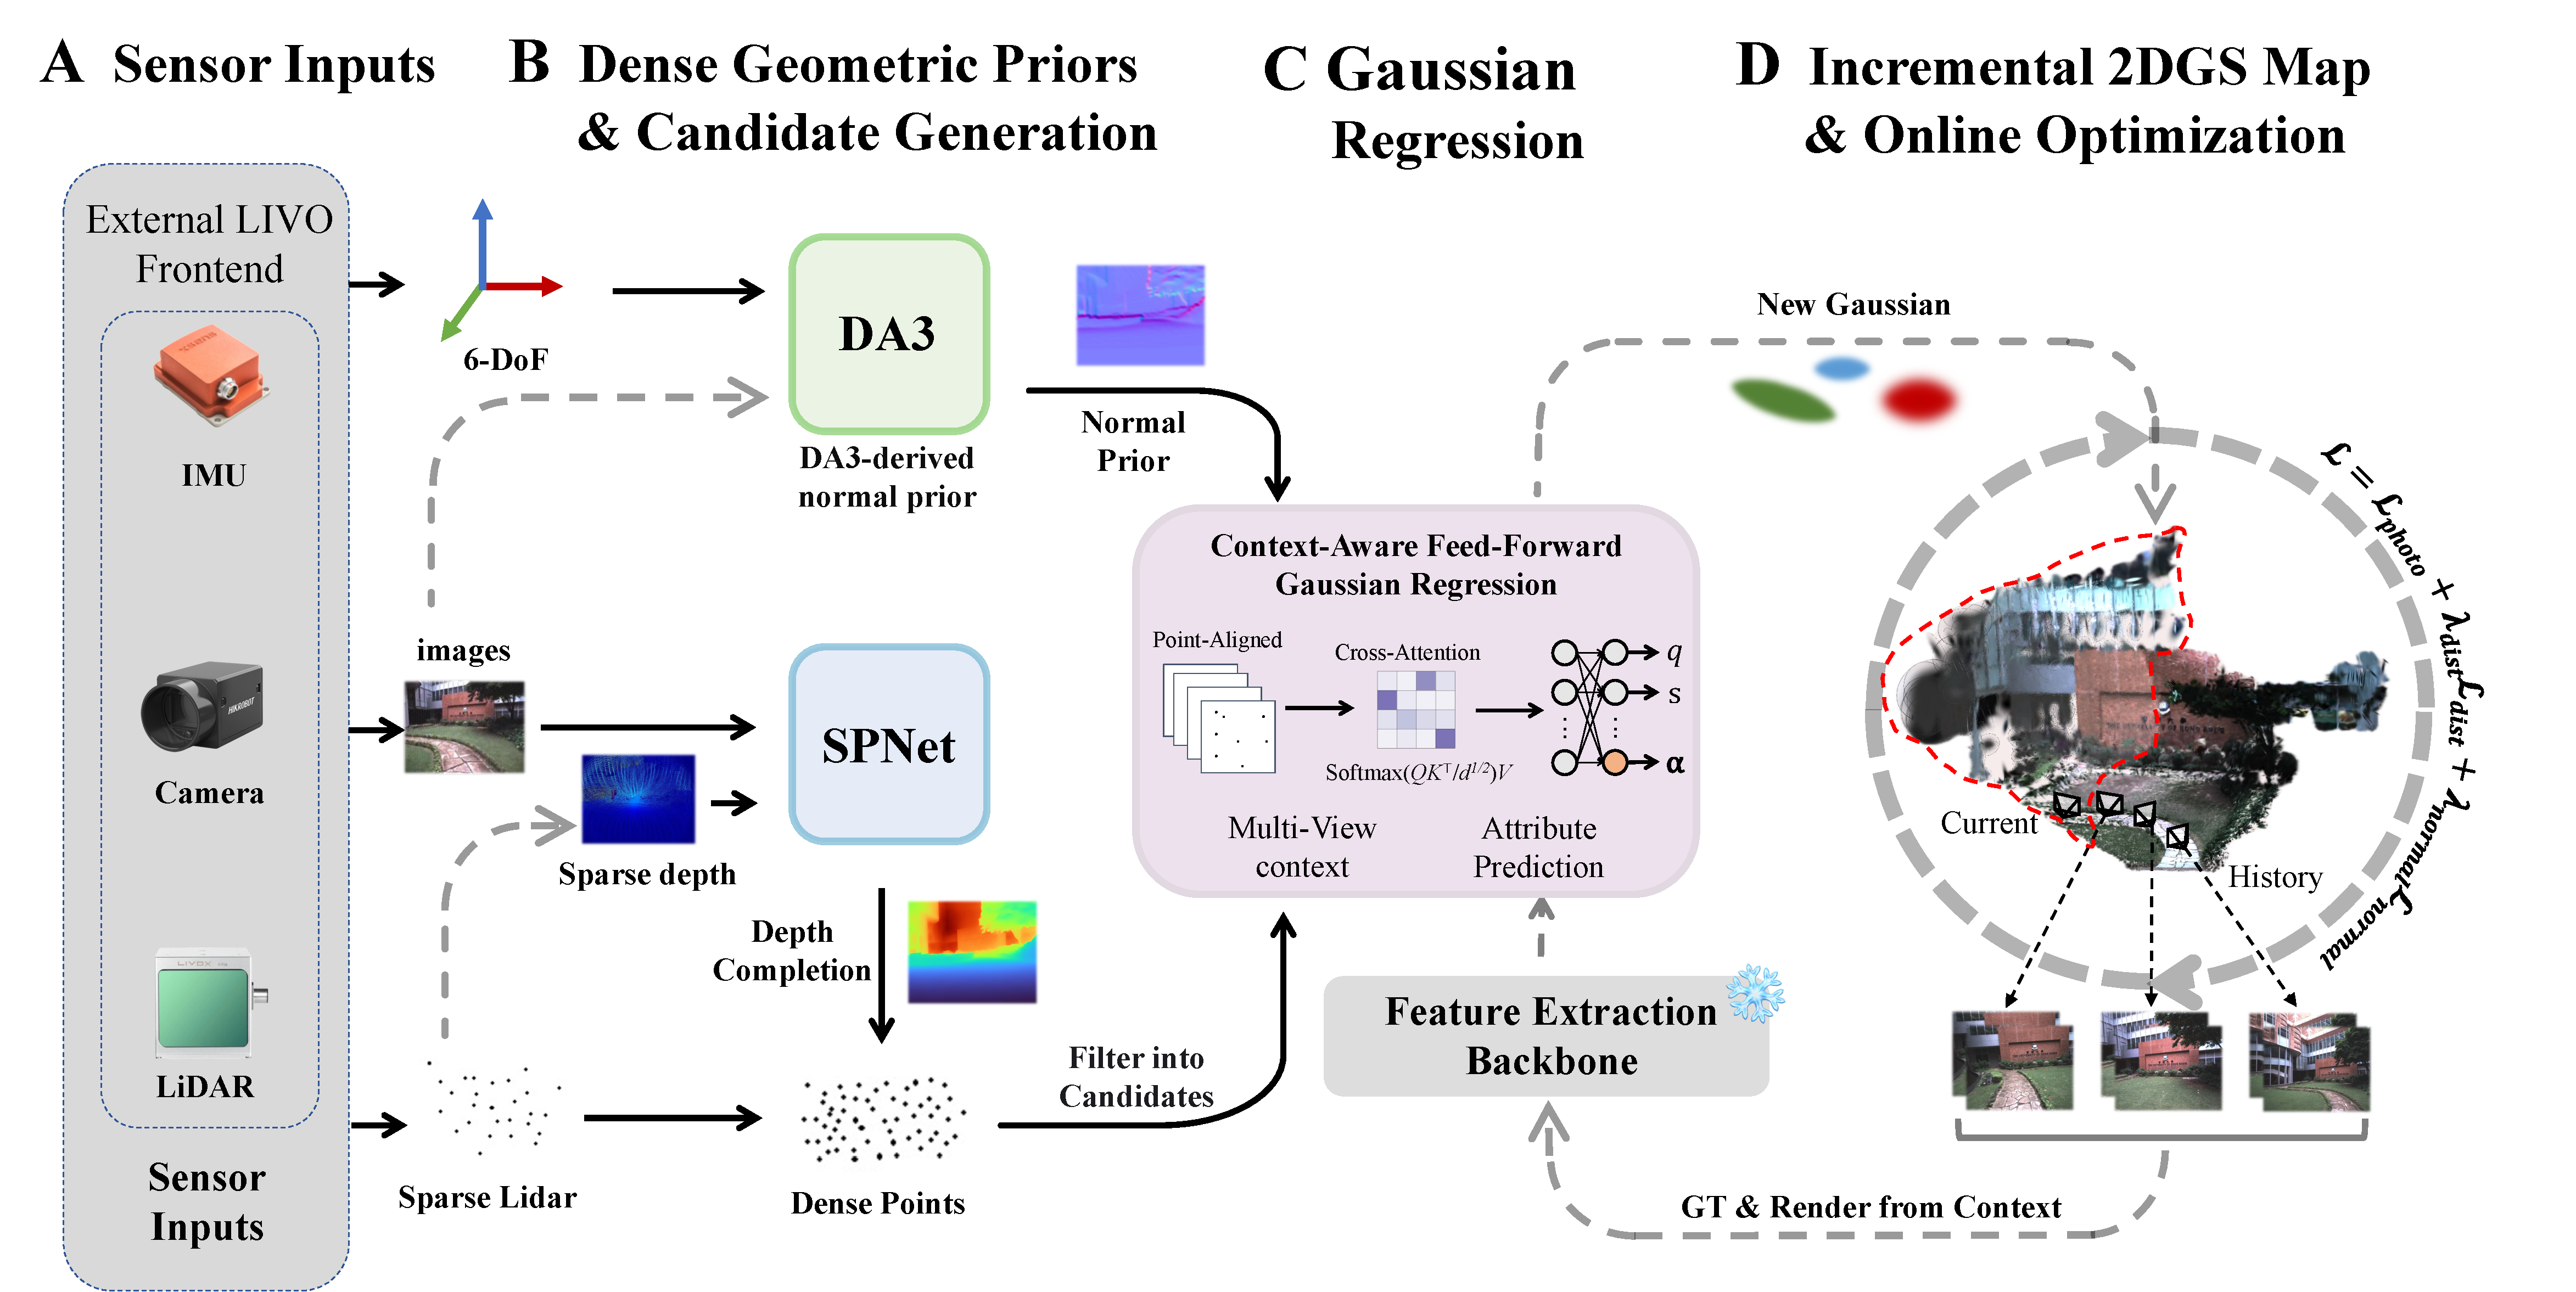
\includegraphics[width=\textwidth,height=0.36\textheight,keepaspectratio]{../../system-pipeline.pdf}
    \caption{系统整体流程。(A) 外部 LiDAR-惯导-视觉前端提供同步的 RGB 图像、LiDAR 观测、IMU 信息和相机位姿。(B) 系统利用 SPNet 深度补全和 DA3 法线估计生成稠密几何先验，并与 LiDAR 点共同形成欠重建区域的初始点。(C) 对于每个候选点，前馈高斯回归器聚合逐点对齐的多视图上下文，直接预测完整的 2DGS surfel 属性。(D) 预测得到的新 surfel 被插入增量地图后，再结合在线优化进一步更新；同时，当前地图的渲染结果继续作为后续插点的上下文输入。}
    \label{fig:system_pipeline}
\end{figure*}

\section{Method}

% IEEEtran 的 \subsubsection/\paragraph 在期刊模板中会生成运行内标题。
% 会议稿直接迁移过来时，中文方法节容易出现异常缩进和重复编号（例如 a) 与手写 (a) 叠加）。
% 因此这里统一改为手工控制的小标题引导样式，保持版式稳定且与模板观感一致。
\providecommand{\methodlead}[1]{\vspace{0.35em}\noindent\textit{#1}}

\subsection{系统概述}

本系统是一个基于外部位姿前端的增量式 2DGS 场景重建后端。系统接收外部 LiDAR-Inertial-Camera 前端（如 R3Live）实时输出的同步数据流，每帧包含 RGB 图像、稀疏 LiDAR 点云和 6-DOF 相机位姿，以 2DGS surfel 为基础地图表示。整体流程如图 X 所示。

当新关键帧到达时，系统首先将稀疏 LiDAR 点投影到图像平面形成稀疏深度图，经 SPNet 深度补全后在 LiDAR 盲区生成补充初始 3D 点；与此同时，DA3 单目深度估计模型预测稠密深度并与 LiDAR 对齐，由此为初始点提供法线先验。在初始点生成后，系统对当前高斯地图进行渲染，依据渲染透明度和颜色误差识别欠重建区域，并结合颜色梯度过滤与体素下采样，从中筛选出确需新增高斯的候选点子集。筛选后的候选点被组织为回归器的两类输入，即上下文特征输入 $\mathbf{ctx}$ 与几何先验输入 $\mathbf{g}$，并送入前馈回归网络。该网络通过跨注意力机制融合多视角上下文，在单次前向传播中直接回归每个候选点的完整 surfel 属性。预测的新高斯插入地图后，系统在滑窗内的关键帧上进行多轮在线优化，以光度损失（L1 + SSIM）与 2DGS 几何约束损失（深度畸变 + 法线一致性）联合驱动高斯属性收敛。非关键帧仅接收位姿而不触发地图扩展。

前馈回归网络的训练通过自蒸馏训练完成。系统首先以 \texttt{naive} 模式（不使用前馈网络，采用传统的基于规则初始化）在训练场景上运行一遍完整的增量式建图；当某帧新增高斯的累积训练次数达到预设阈值后，系统快照其当前属性，并在该时刻构造对应的上下文特征输入 $\mathbf{ctx}$ 与几何先验输入 $\mathbf{g}$，形成训练样本，随后离线训练前馈网络。

\subsection{稠密几何先验}

采用 SPNet 轻量级深度补全网络将 RGB 图像与稀疏 LiDAR 深度融合为稠密深度图，并在无 LiDAR 覆盖的区域采样补充 3D 初始点。最终，SPNet 补充点与原始 LiDAR 投影点合并构成初始点集。

使用 DA3 对当前帧 RGB 图像推理输出相对深度图后，系统通过最小二乘仿射对齐将其与稀疏 LiDAR 深度配准，得到与真实尺度一致的稠密深度图，再以中心差分计算逐像素法线。按初始点的像素坐标在法线图上采样，得到每个初始点的相机空间法线 $\mathbf{n}_{\text{cam}} \in \mathbb{R}^3$。

\subsection{前馈高斯回归网络}

% 网络结构图跟随前馈高斯回归网络小节进入浮动队列，并保持在系统流程图之后编号。
\begin{figure*}[!t]
    \centering
    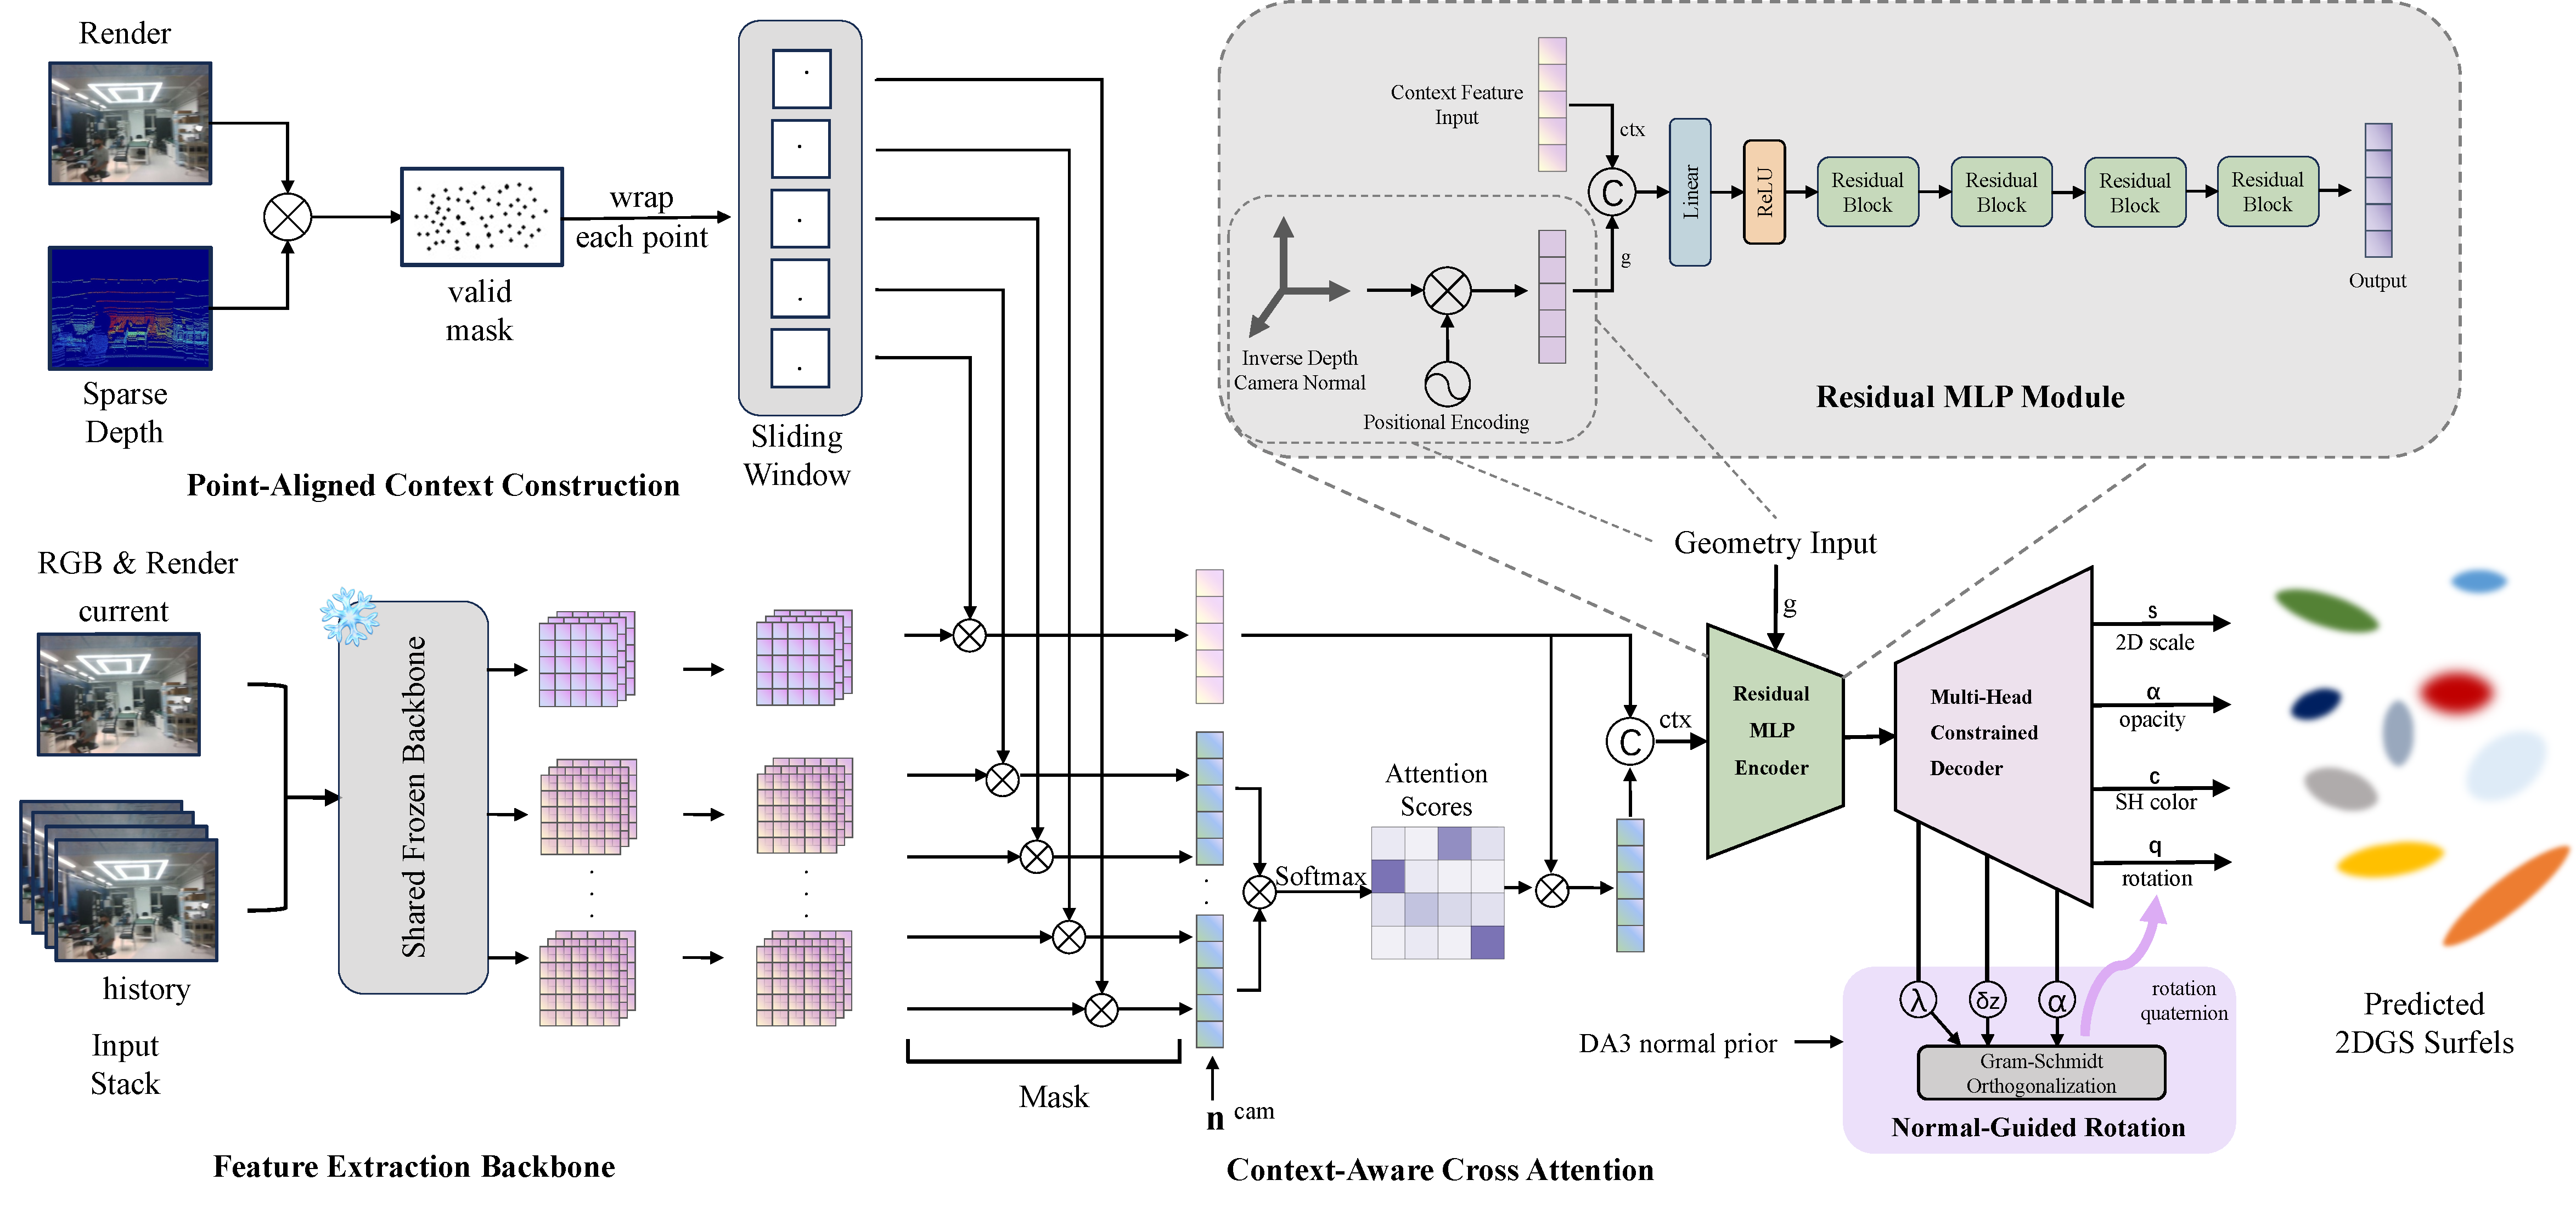
\includegraphics[width=\textwidth,height=0.34\textheight,keepaspectratio]{../../net-pipeline.pdf}
    \caption{上下文感知前馈高斯回归器结构。网络首先在滑动窗口内对有效候选种子构造逐点对齐的上下文，并通过冻结的共享主干提取当前帧与历史帧的图像-渲染特征；随后，跨注意力模块汇聚多视图外观信息，并与逆深度、DA3 法线和位置编码等几何先验一起输入残差 MLP 编码器；最后，多头约束解码器预测完整的 2DGS surfel 属性 $(\mu, s, \alpha, c, q)$，其中法线引导的旋转分支通过 Gram-Schmidt 正交化构造几何一致的朝向。}
    \label{fig:net-pipeline}
\end{figure*}

与 MVSplat 一类直接从多视图图像恢复高斯参数的方法不同，本文关注的是在候选点已经由上游几何模块确定的条件下，学习从上下文特征输入 $\mathbf{ctx}$ 与几何先验输入 $\mathbf{g}$ 到 surfel 参数的映射。对于当前关键帧筛选得到的 $N_t$ 个候选点，记 $\mathbf{ctx}_i$ 为点 $i$ 的上下文特征输入，$\mathbf{g}_i$ 为其几何先验输入，则前馈网络的目标可写为：

\begin{equation}
f_{\boldsymbol{\theta}} : \{(\mathbf{ctx}_i, \mathbf{g}_i)\}_{i=1}^{N_t}
\mapsto
\{(\mathbf{s}_i, \mathbf{q}_i, \alpha_i, \mathbf{c}_i^{\mathrm{dc}}, \mathbf{c}_i^{\mathrm{rest}})\}_{i=1}^{N_t},
\end{equation}

其中输出分别对应 surfel 的二维尺度、旋转、不透明度以及 SH 颜色参数。

\methodlead{1) 上下文特征输入 $\mathbf{ctx}$：}与 pixelSplat、MVSplat 等需要同时恢复几何与外观的离线方法不同，本文候选点位置已由上游几何模块确定，网络只需围绕每个候选点构造逐点对齐的多视图上下文。共享 backbone（沿用 pixelSplat 设计，训练时冻结）分别对当前帧原始图像、当前帧渲染图像以及滑窗内 $W$ 帧历史关键帧的原始与渲染图像提取特征图。其中渲染图像使网络能显式感知当前地图的重建状态，其与原始图像的差异隐式反映欠重建程度。对每个候选点，系统以其像素坐标在上述特征图上双线性插值采样，并计算归一化观察方向，得到当前帧逐点特征 $\mathbf{f}_i^{\text{curr}}, \mathbf{f}_i^{\text{ren}} \in \mathbb{R}^{D}$ 及历史帧特征 $\mathbf{f}_i^{\text{hist}} \in \mathbb{R}^{W \times D}$；不可见的历史视角由可见性掩码 $\mathbf{m}_i^{\text{hist}} \in \{0,1\}^{W}$ 标记。随后，系统使用跨注意力模块将可变长度的历史观测压缩为固定维度的时序上下文，其中不可见视角在 softmax 前以 $-\infty$ 掩码排除：

\begin{equation}
\mathbf{ctx}_i^{\text{attn}} = \text{softmax}\!\left(\frac{\mathbf{q}_i \mathbf{K}_i^\top}{\sqrt{d_k}} + \mathbf{M}_i\right) \mathbf{V}_i
\end{equation}

\noindent 聚合完成后，当前帧原始特征、渲染特征与 $\mathbf{ctx}_i^{\text{attn}}$ 拼接，构成送入编码器的上下文特征 $\hat{\mathbf{ctx}}_i$。

\methodlead{2) 几何先验输入 $\mathbf{g}$：}几何先验输入由逆深度、DA3 相机空间法线、有效性掩码和 KNN 像素间距拼接得到：
\begin{equation}
\mathbf{g}_i = [\bar{z}_i^{-1} \| \mathbf{n}_i^{\text{cam}} \| m_i \| d_i^{\text{nn}}].
\end{equation}

\noindent 其中 $\bar{z}_i^{-1}$ 提供尺度恢复所需的深度信息，$\mathbf{n}_i^{\text{cam}}$ 为 surfel 朝向的法线锚点，$m_i$ 标记几何先验是否有效，$d_i^{\text{nn}}$ 刻画局部采样密度。各连续分量经 NeRF 风格位置编码后与 $\hat{\mathbf{ctx}}_i$ 拼接，送入由一层线性投影和 4 个 pre-activation 残差块构成的编码器，输出 512 维隐变量 $\mathbf{h}_i$。

\methodlead{3) 回归器解码器：}在共享隐变量 $\mathbf{h}_i$ 的基础上，系统使用多个独立预测头以 $\text{Linear} \to \text{ReLU} \to \text{Linear}$ 的形式回归不同属性。各头输出并不直接作为最终高斯参数，而是结合上游几何先验进行约束解码，从而使预测结果更稳定地锚定在已有几何信息上。

\methodlead{a) 法线引导的旋转解码：}系统不直接回归四元数，而是以 DA3 提供的相机空间法线 $\mathbf{n}_i^{\text{cam}}$ 为锚点，由网络预测修正量，并通过正交化过程构造完整旋转。网络首先预测法线修正向量 $\delta \mathbf{z}_i \in \mathbb{R}^3$、混合强度 $\lambda_i = \text{softplus}(\cdot) \in \mathbb{R}_{>0}$ 以及辅助向量 $\mathbf{a}_i \in \mathbb{R}^3$，进而得到修正后的法线方向：

\begin{equation}
\mathbf{z}_i = \text{normalize}(\mathbf{n}_i^{\text{cam}} + \lambda_i \cdot \delta \mathbf{z}_i)
\end{equation}

随后利用 Gram-Schmidt 正交化过程构造完整正交基：
\begin{equation}
\mathbf{y}_i = \text{normalize}(\mathbf{z}_i \times \mathbf{a}_i), \qquad \mathbf{x}_i = \mathbf{y}_i \times \mathbf{z}_i.
\end{equation}

最终，相机系旋转矩阵 $[\mathbf{x}_i \mid \mathbf{y}_i \mid \mathbf{z}_i]$ 经当前帧位姿 $R_{\text{wc}}$ 转换到世界系，并转为四元数存储。

\methodlead{b) 密度自适应尺度解码：}尺度头预测 surfel 在像素平面上的相对尺度，并通过局部点密度先验进行调节：
\begin{equation}
\mathbf{s}_i^{\text{pixel}} = \frac{d_i^{\text{nn}}}{2} \cdot \exp(\text{head}(\mathbf{h}_i)) \in \mathbb{R}^2_{>0}.
\end{equation}

其中 $d_i^{\text{nn}}$ 为候选点的 KNN 像素间距。最终世界空间尺度由
\begin{equation}
\mathbf{s}_i^{\text{world}} = \mathbf{s}_i^{\text{pixel}} / (\bar{z}_i^{-1} \cdot f)
\end{equation}
恢复得到。该参数化避免了网络直接学习深度相关的绝对尺度，而只需学习与局部密度相关的相对尺度变化。

\methodlead{c) 颜色解码：}DC 颜色头输出残差 $\Delta \mathbf{c}_i^{\text{dc}}$，并加到由单帧 RGB 观测转换得到的基础 SH 先验上，形成
\begin{equation}
\mathbf{c}_i^{\text{dc}} = \text{RGB2SH}(\mathbf{I}_i) + \Delta \mathbf{c}_i^{\text{dc}}.
\end{equation}
高阶 SH 系数则由独立头直接预测。该残差设计使网络能够从合理的颜色先验出发，仅学习局部修正量。

\methodlead{d) 不透明度解码：}不透明度头经 sigmoid 激活输出 $\alpha_i \in (0,1)$，随后转为 logit 空间存储。

\subsection{自蒸馏训练}

前馈网络的训练不依赖外部多视图标注数据集，而是通过以下自蒸馏管线完成。

\methodlead{1) 在线数据采集：}系统首先以 \texttt{naive} 模式（不使用前馈网络，而采用基于规则的初始化）在训练场景上运行一次完整的增量式建图。运行过程中，当某帧新增高斯的累积训练次数达到预设阈值时，系统快照这些高斯在该时刻的属性作为监督信号；与此同时，将它们投影到当前滑动窗口中，按照前文定义构造对应的上下文特征输入 $\mathbf{ctx}_i$ 与几何先验输入 $\mathbf{g}_i$。

因此，采集产物以高斯为核心单位组织，每个训练样本都可直接写成前文定义的输入输出对 $(\mathbf{ctx}_i, \mathbf{g}_i) \mapsto (\mathbf{s}_i, \mathbf{q}_i, \alpha_i, \mathbf{c}_i^{\mathrm{dc}}, \mathbf{c}_i^{\mathrm{rest}})$。

\methodlead{2) 尺度-旋转歧义消解：}2DGS surfel 存在固有的尺度-旋转歧义：交换两个切线方向的尺度并相应旋转 $90^\circ$ 可得到等价表示。若不消解此歧义，训练标签中同一几何形态会对应两种不同的参数组合，导致网络学习不稳定。

数据准备阶段显式消解此歧义：对每个 GT 高斯，强制 $s_1 \geq s_2$；当需要交换时，同步对四元数施加 $90^\circ$ 旋转：$\mathbf{q}' = \text{normalize}((w-z, x+y, y-x, w+z) / \sqrt{2})$。

\methodlead{3) 训练目标：}网络以多任务损失联合训练，涵盖尺度、旋转、颜色和不透明度全部预测属性。尺度损失在 log 世界尺度空间以 L1 距离度量；旋转损失采用四元数余弦距离 $\mathcal{L}_{\text{rot}} = 1 - |\langle \mathbf{q}_{\text{pred}}, \mathbf{q}_{\text{gt}} \rangle|$；颜色损失对 DC 和高阶 SH 系数分别以 MSE 监督；不透明度损失为 L1 距离。
  